\section{Desenvolvimento dos Osciladores em Anel}
\label{sec:MetOscilador}

A topologia de oscilador em anel foi escolhida para os testes por sua disseminada utilização na caracterização de dispositivos MOSFET. Seu uso é amplo, pois medidas utilizando esse circuito se aproximam muito mais de aplicações reais do que medições paramétricas DC padrões.

Foram realizados testes preliminares com diferentes quantidades de inversores para encontrar uma quantidade apropriada, pois, com poucos osciladores a capacitância de saída afeta demais o sinal, o que faz com que ele não seja mais uma onda quadrada e com muitos osciladores o limite de iterações em um bloco 'for' que as IDEs permitem era atingido.

Considerando isso, foi decidido que em cada um dos dispositivos seria sintetizado dois osciladores, um com 1001 inversores, pois foi o valor em que se considerou que a onda poderia ser considerada quadrada, e outro com 4999, por ser o maior valor ímpar permitido pela IDE Quartus II. A escolha de utilizar dois osciladores em cada FPGA foi tomada por dois motivos: para se ter certeza que as IDEs não estavam simplificando os estágios inversores do circuito sintetizado e para verificar que o envelhecimento afeta igualmente diferentes partes do FPGA.

A grande quantidade de inversores é relevante, pois assim as pequenas variações aleatórias nas características de cada transistor que compõe os dispositivos tenderão a se diluir.

\subsection{Desenvolvimento do Código para os Osciladores}

Para desenvolver e sintetizar os osciladores em anel foi utilizada a linguagem de descrição Verilog. Para o Cyclone II foi utilizada a IDE Quartus II versão 12.1, já para o ZedBoard foi utilizada a IDE Vivado versão 2023.1.

O Quadro \ref{code:RingOsc} mostra o código desenvolvido em Verilog para o módulo que implementa o oscilador em anel com N inversores, sendo N igual a 5 caso nenhum valor seja definido durante a instanciação do módulo. O mesmo código foi utilizado para os dois FPGAs nas duas IDEs diferentes.

\begin{lstlisting}[label={code:RingOsc}, style=VerilogStyle, caption={Módulo do Oscilador em Anel. Fonte: O Autor}]
module RingOscillator 
	#(parameter N = 5)
	(
		input  en,
		output reg and_1    /*synthesis keep*/
	);
	reg [N - 1:0] notGate /*synthesis keep*/;
	integer i;
	generate
	  always @ (*) begin
		  and_1 <= en & notGate[N - 1];
	  	notGate[0] <= ~and_1;
	  	for (i = 1; i < N; i = i + 1)   begin: inverter_chain
			  notGate[i] <= ~notGate[i - 1];
		  end
	  end
	endgenerate
endmodule
\end{lstlisting}

O módulo possui uma entrada en, responsável por habilitar o circuito, uma saída and\_1 que é a saída da porta and do circuito, de onde o sinal do oscilador é obtido. O valor N é parametrizável, o que permite a reutilização do mesmo código para osciladores com diferentes números de inversores.

São então instanciadas N variáveis, que serão utilizados para criar os inversores. A variável and\_1 recebe o resultado da operação E lógica do sinal de \textit{enable} e a saída do último inversor. O primeiro inversor é definido como a variável and\_1 invertido.

Um bloco 'for' é utilizado para automatizar as atribuições dos inversores seguintes, sendo a cada um atribuído o valor inversor anterior negado.

Um ponto importante de destacar é a necessidade de utilizar diretivas de compilação para impedir que os inversores sejam simplificados na síntese. Essas diretivas são diferentes em cada uma das IDEs, na Quartus II é utilizado a diretiva /* synthesis keep */ e na Vivado é utilizado a diretiva /* synthesis syn\_keep=1 */.

% Na Figura \ref{fig:DE2Imp3Osc} pode ser visto como o Quartus II implementa em hardware o código do Quadro \ref{code:RingOsc} para um N igual a 3. A implementação é feita através de portas lógicas comuns, o que é diferente da implementação feita pelo Vivado, como visto na Figura \ref{fig:ZedImp3Osc}, que utiliza LUTs de uma variável para representar os inversores.

Nas Figuras \ref{fig:DE2Imp3Osc} e \ref{fig:ZedImp3Osc} pode ser visto como, respectivamente, o Quartus II e o Vivado implementam em hardware o código do quadro \ref{code:RingOsc} para um N igual a 3. É importante destacar que, por mais que para o Quartus II sejam utilizados portas lógicas para ilustrar o circuito, essas portas lógicas são construídas, na verdade, com LUTs que implementam o seu comportamento.

\begin{figure}[H]
    \centering
    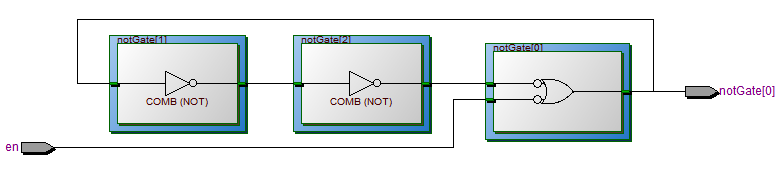
\includegraphics[width=\linewidth]{figures/Metodologia/DE2_Implementation_3Inverter_Gates.png}
    \caption{Síntese de um oscilador com três inversores no Quartus II. Fonte: O Autor}
    \label{fig:DE2Imp3Osc}
\end{figure}

\begin{figure}[H]
    \centering
    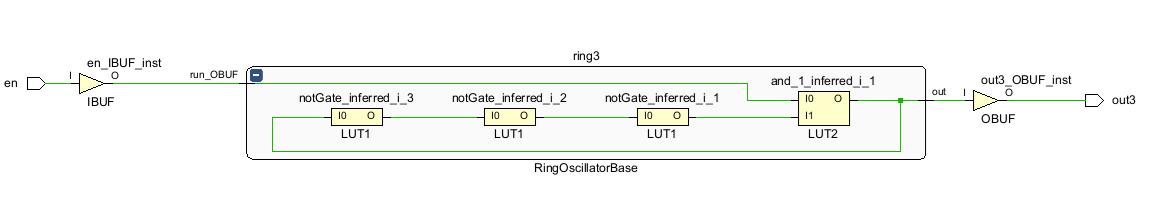
\includegraphics[width=\linewidth]{figures/Metodologia/ZedBoard_Implementation_3Inverter.png}
    \caption{Síntese de um oscilador com três inversores gerado no Vivado. Fonte: O Autor}
    \label{fig:ZedImp3Osc}
\end{figure}

O Quadro \ref{code:TopLevel} mostra o módulo de alto nível em que é instanciado dois osciladores em anel, um com 1001 e outro de 4999 inversores. 

\begin{lstlisting}[label={code:TopLevel}, style=VerilogStyle, caption={Instanciação dos Módulos. Fonte: O Autor}]
module TopLevel
	(
		input en,
		output run,
		output out1001, out4999
	);
	
	assign run = en;

	RingOscillator #(.N(1001)) ring1001(en, out1001);
	RingOscillator #(.N(4999)) ring4999(en, out4999);
endmodule
\end{lstlisting}

O módulo possui uma entrada 'en', responsável por habilitar o circuito, uma saída 'run', usada para indicar que o circuito está em funcionamento e as saídas dos dois osciladores 'out1001', 'out4999'. Também são declaradas duas instâncias do módulo desenvolvido no Quadro \ref{code:RingOsc}.

As Figuras \ref{fig:DE2RtlSchem} e \ref{fig:ZedRtlSchem1} mostram, respectivamente, o circuito implementado pelo software Quartus II e Vivado para o módulo de alto nível que serão utilizado nos FPGAs.

\begin{figure}[H]
    \centering
    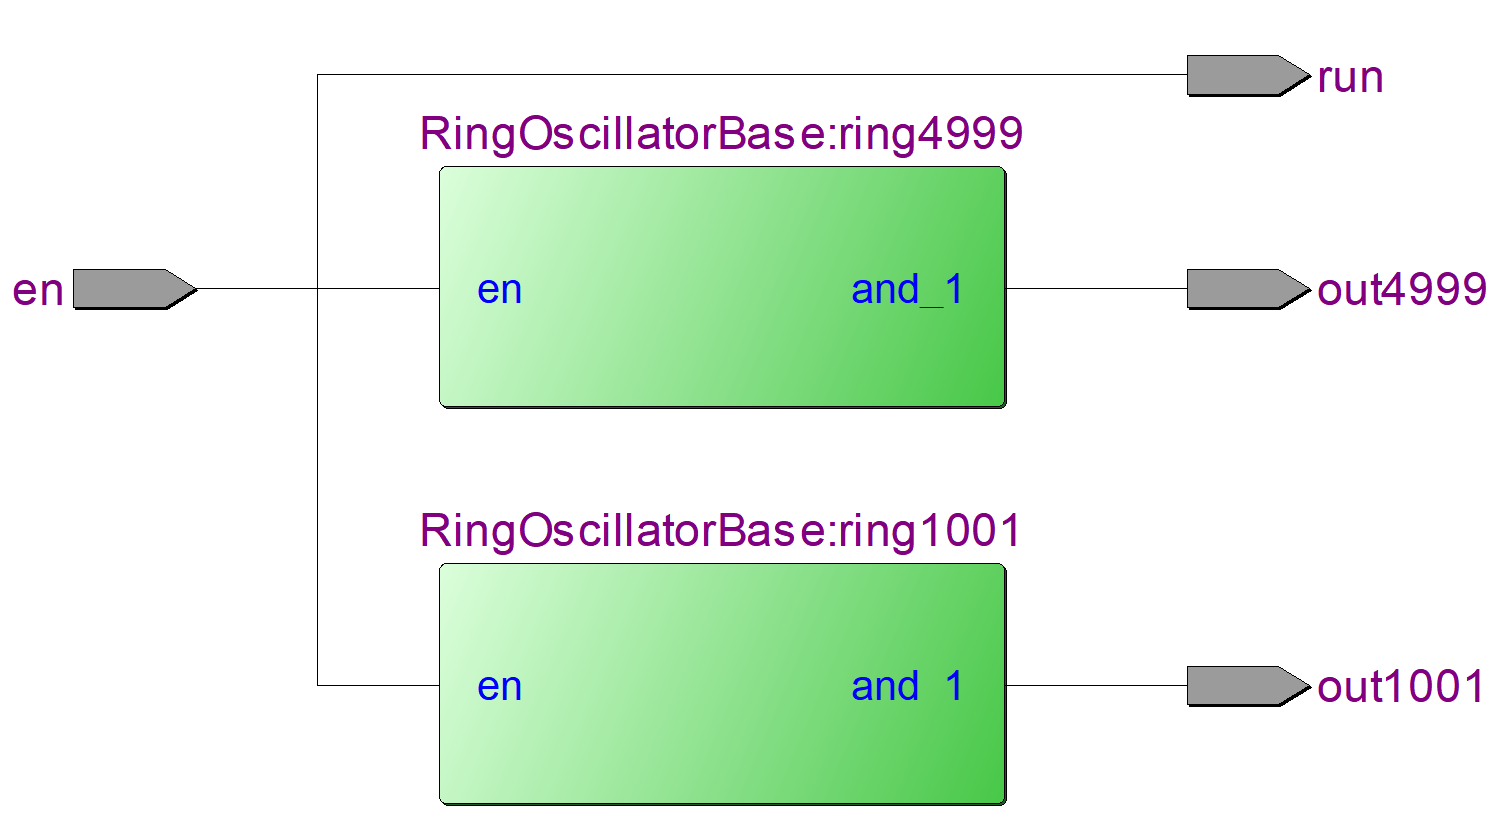
\includegraphics[scale=0.25]{figures/Metodologia/DE2_RTL_Schematic.png}
    \caption{Síntese do módulo de alto nível gerado no Quartus II. Fonte: O Autor}
    \label{fig:DE2RtlSchem}
\end{figure}

\begin{figure}[H]
    \centering
    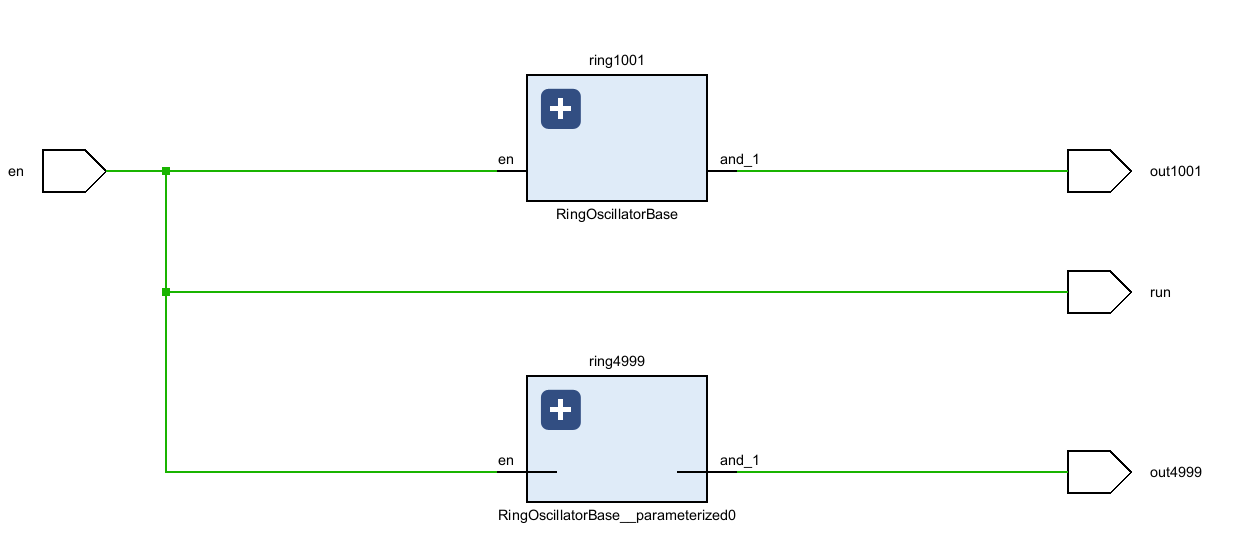
\includegraphics[width=\linewidth]{figures/Metodologia/ZedBoard_RTL_Schematic.png}
    \caption{Síntese do módulo de alto nível gerado no Vivado. Fonte: O Autor}
    \label{fig:ZedRtlSchem1}
\end{figure}

Nas duas placas a entrada 'en' foi atribuída a um pino do FPGA ligado a uma chave, a saída 'run' foi atribuída a um pino do FPGA ligado a um LED e as saídas 'out1001' e out4999 foram atribuídas a pinos do FPGA ligados a conectores de entrada e saída de uso geral.

Em ambas as sínteses foram utilizadas 6000 elementos lógicos, quantidade condizente com inversores presentes em cada um dos dois osciladores. Isso mostra que a única simplificação que ocorreu foi a operação lógica E ter sido integrada ao primeiro inversor da corrente.

Após o desenvolvimento, o circuito sintetizado foi simulado utilizando a ferramenta apropriada para cada um dos componentes. Constatada a validade da solução ela foi transferida para os FPGAs reais e será medida, através de um osciloscópio, a frequência de oscilação das saídas do circuitos.